\documentclass[11pt,a4paper]{article}

\usepackage[margin=1in]{geometry}
\usepackage[T1]{fontenc}
\usepackage{lmodern}
\usepackage{microtype}
\usepackage{setspace}
\usepackage{longtable}
\usepackage{array}
\usepackage{booktabs}
\usepackage{tabularx}
\usepackage{enumitem}
\usepackage{xcolor}
\usepackage{hyperref}
\usepackage{tikz}
\usepackage{listings}
\usepackage{graphicx}
\graphicspath{{images_sds/}}
\usetikzlibrary{shapes.geometric,arrows.meta,positioning,fit,backgrounds,calc,chains,shapes.multipart,shapes.symbols}

\hypersetup{
    colorlinks=true,
    linkcolor=blue!60!black,
    urlcolor=blue!60!black,
}

\onehalfspacing
\setlength{\parskip}{0.5em}
\setlength{\parindent}{0pt}
\renewcommand{\arraystretch}{1.25}
\newcolumntype{L}[1]{>{\raggedright\arraybackslash}p{#1}}

\lstset{
    basicstyle=\ttfamily\footnotesize,
    breaklines=true,
    frame=single,
    columns=fullflexible,
}

% TikZ styles
\tikzset{
    tier/.style={rectangle, draw, thick, minimum width=10cm, minimum height=1.4cm, align=center, font=\small, fill=blue!5},
    entity/.style={rectangle, draw, thick, rectangle split, rectangle split parts=2, align=center, font=\small\ttfamily, fill=yellow!10},
    class/.style={rectangle, draw, thick, rectangle split, rectangle split parts=3, align=left, font=\scriptsize\ttfamily, text width=4.6cm, fill=green!5},
    state/.style={rectangle, draw, thick, rounded corners=6pt, minimum width=2.2cm, minimum height=0.8cm, align=center, font=\small, fill=blue!8},
    activity/.style={rectangle, draw, thick, rounded corners=10pt, minimum width=4cm, minimum height=0.75cm, align=center, font=\footnotesize, fill=orange!10},
    decision/.style={diamond, draw, thick, aspect=2, align=center, font=\footnotesize, fill=red!8},
    start/.style={circle, draw, thick, fill=black, minimum size=4mm, inner sep=0},
    endst/.style={circle, draw, thick, double, minimum size=4mm, inner sep=0},
    lifeline/.style={dashed, thick},
    msg/.style={-{Stealth[length=2mm]}, thick},
    flow/.style={-{Stealth[length=2.5mm]}, thick},
    box/.style={rectangle, draw, thick, minimum height=0.8cm, align=center, font=\small, fill=blue!8},
    screen/.style={rectangle, draw, thick, minimum width=10cm, minimum height=6.5cm, fill=gray!3},
    sbox/.style={rectangle, draw, thin, font=\footnotesize, align=center, fill=white},
}

\title{\textbf{Software Design Specification} \\[0.4em] \large SwishVision: Basketball Analytics Platform}
\author{Mallick Mikaal Imam \and Minhaj ul Hassan \and Muhammad Ahmed Silat \and Syed Muhammad Sameer Hassan}
\date{Version 1.10 \\ 11th May 2026}

\begin{document}

\maketitle
\thispagestyle{empty}

\begin{center}
\begin{tabular}{|L{6cm}|L{6cm}|}
\hline
\textbf{Project Team} & \\ \hline
Mallick Mikaal Imam & \\ \hline
Minhaj ul Hassan & \\ \hline
Muhammad Ahmed Silat & \\ \hline
Syed Muhammad Sameer Hassan & \\ \hline
\end{tabular}

\vspace{0.5em}
\begin{tabular}{|L{6cm}|L{6cm}|}
\hline
\textbf{Submission Date} & 11th May 2026 \\ \hline
\end{tabular}
\end{center}

\newpage

\section*{Document History}
\begin{longtable}{|c|L{3.5cm}|L{2.8cm}|L{6.5cm}|}
\hline
\textbf{Version} & \textbf{Name} & \textbf{Date} & \textbf{Description of Change} \\ \hline
1.00 & Ahmed Silat & 16 Mar 2026 & Initial draft, architecture and design documented \\ \hline
1.10 & Minhaj ul Hassan & 11 May 2026 & Post-implementation update, finalised technology stack table, replaced PostgreSQL with SQL Server (pyodbc), updated file system layout to match shipped \texttt{app/} structure, updated environment variables \\ \hline
1.11 & Minhaj ul Hassan & 11 May 2026 & Corrected output codec across the document, pipeline writes H.264 \texttt{.mp4} (via \texttt{mp4v} then \texttt{imageio-ffmpeg} transcode). Updated output filename pattern to actual \texttt{output\_session\_\{id\}\_\{n\}\_processed.mp4}. \\ \hline
\end{longtable}

\section*{Document Information}
\begin{tabular}{|L{4cm}|L{10cm}|}
\hline
Project & SwishVision \\ \hline
Document & Software Design Specification \\ \hline
Document Version & 1.10 \\ \hline
Status & Final \\ \hline
Author(s) & Mallick Mikaal Imam, Minhaj ul Hassan, Muhammad Ahmed Silat, Syed Muhammad Sameer Hassan \\ \hline
Approver(s) & Course Supervisor \\ \hline
\end{tabular}

\newpage
\tableofcontents
\newpage

\section{Introduction}

\subsection{Purpose of Document}
This document provides the design specifications for SwishVision. It outlines both the high-level architectural view and the detailed low-level design of the system, covering the web platform, the CV processing pipeline, data models, and their interactions. The document serves as the blueprint that guides implementation and ensures alignment between design decisions and the requirements stated in the SRS.

\subsection{Intended Audience}
This document is intended for the development team building the system, the course supervisor evaluating the design, and any future maintainers.

\subsection{Document Convention}
\begin{itemize}[leftmargin=*]
    \item Font: Arial (Latin Modern as LaTeX substitute)
    \item Size: 11
    \item Line Spacing: 1.5
\end{itemize}

\subsection{Project Overview}
SwishVision is a web-based analytics platform that transforms basketball practice footage into structured performance data using computer vision and pose estimation. A fully working CLI prototype already exists, built on YOLOv8 for object detection and pose estimation. The object detection model (\texttt{best.pt}) was fine-tuned from YOLOv8 over 13 training iterations on the Basketball-1 Roboflow dataset. Human pose estimation uses \texttt{yolov8m-pose.pt}, tracking 17 body keypoints.

The design objective of this phase is to wrap that pipeline in a web application, adding user management, video upload, asynchronous processing, and a results dashboard.

The pipeline executes 12 steps: (1) frame extraction, (2) ball detection (\texttt{BallTracker}), (3) rim detection (\texttt{RimTracker}), (4) pose detection (\texttt{HumanTracker}), (5) track validation, (6) trajectory interpolation, (7) joint angle calculation, (8) ball-hand interaction (\texttt{ball\_hand()}), (9) shot start identification (\texttt{shot\_started()}), (10) frame annotation, (11) shot outcome detection (\texttt{ShotTracker}), and (12) output video write and report generation.

\subsection{Scope}
\begin{itemize}[leftmargin=*]
    \item Design of the web application layer (frontend + backend API)
    \item Design of the user authentication subsystem
    \item Design of the video upload and storage subsystem
    \item Design of the asynchronous job queue for video processing
    \item Design of the database schema
    \item Integration design between the web layer and the existing CLI pipeline
    \item Design of the results dashboard and reporting views
\end{itemize}

\section{Design Considerations}

\subsection{Assumptions and Dependencies}
\begin{itemize}[leftmargin=*]
    \item Existing pipeline modules (\texttt{BallTracker}, \texttt{RimTracker}, \texttt{HumanTracker}, \texttt{ShotTracker}, drawers) are stable internal libraries, invoked by a worker, not modified.
    \item Pre-trained model files are available under \texttt{models/}: \texttt{best.pt} ($\sim$43\,MB) and \texttt{yolov8m-pose.pt} ($\sim$78\,MB).
    \item Additional model variants (\texttt{bestOld.pt}, \texttt{bestYT.pt}, \texttt{ballRim.pt}) exist but are not used in the primary pipeline.
    \item Video storage is local filesystem-based for the current version.
    \item A Microsoft SQL Server 2019+ instance is available with the appropriate ODBC driver.
    \item The task queue uses Celery with Redis as broker.
    \item Output videos are written in two stages: \texttt{mp4v} via OpenCV, then transcoded to H.264 (\texttt{libx264}, \texttt{yuv420p}, \texttt{+faststart}) using \texttt{imageio-ffmpeg}.
    \item Intermediate data files (\texttt{angs.txt}, \texttt{xy\_coords.txt}, \texttt{detections.txt}, \texttt{ball\_locl.txt}) are transient.
    \item \texttt{stubs\_utils.py} can cache and reload intermediate tracking results.
\end{itemize}

\subsection{Risks and Volatile Areas}
\begin{itemize}[leftmargin=*]
    \item \textbf{Model output variability:} Accuracy varies with video quality, lighting, and angle.
    \item \textbf{Processing time unpredictability:} Inference time varies; the async queue decouples upload from results.
    \item \textbf{File storage growth:} Videos and outputs can be large; retention policy required.
    \item \textbf{Interpolation artefacts:} \texttt{interpolate\_missing\_tracks()} can produce false positives.
    \item \textbf{Shot start detection sensitivity:} \texttt{shot\_started()} depends on pose keypoints and ball-hand distance.
    \item \textbf{Multiple model variants:} Web layer must use \texttt{best.pt} as the canonical production model.
\end{itemize}

\section{System Architecture}

\subsection{System Level Architecture}

SwishVision follows a three-tier architecture: a client browser communicates with the Web Application Server over HTTPS; processing is offloaded to a Background Worker via a task queue; the worker writes results to the database and filesystem.

\begin{center}
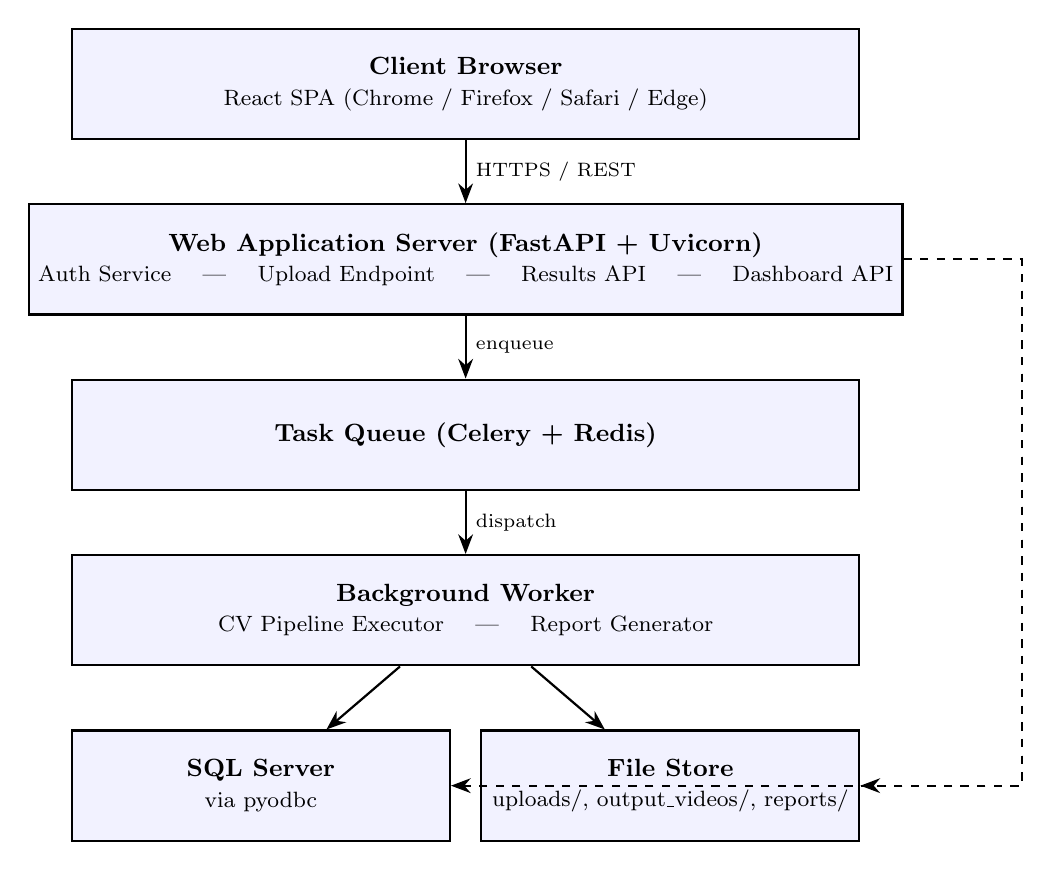
\begin{tikzpicture}[node distance=0.8cm]
    \node[tier] (client) {\textbf{Client Browser} \\ \footnotesize React SPA (Chrome / Firefox / Safari / Edge)};
    \node[tier, below=of client] (web) {\textbf{Web Application Server (FastAPI + Uvicorn)} \\ \footnotesize Auth Service \quad | \quad Upload Endpoint \quad | \quad Results API \quad | \quad Dashboard API};
    \node[tier, below=of web] (queue) {\textbf{Task Queue (Celery + Redis)}};
    \node[tier, below=of queue] (worker) {\textbf{Background Worker} \\ \footnotesize CV Pipeline Executor \quad | \quad Report Generator};
    \node[tier, below=of worker, minimum width=4.8cm, xshift=-2.6cm] (db) {\textbf{SQL Server} \\ \footnotesize via pyodbc};
    \node[tier, below=of worker, minimum width=4.8cm, xshift=2.6cm] (fs) {\textbf{File Store} \\ \footnotesize uploads/, output\_videos/, reports/};

    \draw[flow] (client) -- node[right, font=\scriptsize] {HTTPS / REST} (web);
    \draw[flow] (web) -- node[right, font=\scriptsize] {enqueue} (queue);
    \draw[flow] (queue) -- node[right, font=\scriptsize] {dispatch} (worker);
    \draw[flow] (worker) -- (db);
    \draw[flow] (worker) -- (fs);
    \draw[flow, dashed] (web.east) -- ++(1.5,0) |- (db.east);
    \draw[flow, dashed] (web.east) -- ++(1.5,0) |- (fs.east);
\end{tikzpicture}

\textit{Figure 1: System Architecture}
\end{center}

\subsection{Software Architecture}

\subsubsection{Module Decomposition}

\textbf{1. Auth Module}: registration, login, session management. Exposes \texttt{POST /api/register}, \texttt{POST /api/login}, \texttt{POST /api/logout}.

\textbf{2. Video Module}: upload, storage, lifecycle. Exposes \texttt{POST /api/sessions/upload}, \texttt{GET /api/sessions}, \texttt{GET /api/sessions/\{id\}}, \texttt{DELETE /api/sessions/\{id\}}.

\textbf{3. Processing Module (Worker)}: Celery task that invokes the CV pipeline.

\textbf{4. CV Pipeline (existing)}: trackers, drawers, utils. No direct web exposure.

\textbf{5. Report Module}: structures pipeline output for API responses. Exposes \texttt{GET /api/sessions/\{id\}/report}, \texttt{GET /api/sessions/\{id\}/shots}.

\textbf{6. Dashboard Module}: aggregates session data. Exposes \texttt{GET /api/dashboard/summary}, \texttt{GET /api/dashboard/trends}.

\textbf{7. Frontend}: React UI consuming the REST API. Key views: Landing/Login, Registration, Dashboard, Upload, Session Results, History.

\subsubsection{Technology Stack}

\begin{longtable}{|L{4cm}|L{10cm}|}
\hline
\textbf{Layer} & \textbf{Technology} \\ \hline
Frontend & React 18 (Create React App), JavaScript, Node.js 18+ dev server \\ \hline
Backend Framework & FastAPI 0.135 on Uvicorn 0.42 (ASGI) \\ \hline
ORM / Migrations & SQLAlchemy 2.0 + Alembic 1.14 \\ \hline
Task Queue & Celery 5.6 (worker with \texttt{--pool=solo} on Windows) \\ \hline
Message Broker & Redis 7+ (\texttt{redis://localhost:6379/0}) \\ \hline
Database & Microsoft SQL Server 2019+ via \texttt{pyodbc} (\texttt{mssql+pyodbc}, ODBC Driver 17) \\ \hline
CV Pipeline & Python 3.8+, PyTorch $\geq$2.0, Ultralytics YOLOv8 $\geq$8.0, OpenCV $\geq$4.8 \\ \hline
Authentication & JWT (HS256) via \texttt{python-jose}; passwords hashed with \texttt{bcrypt} (\texttt{passlib}) \\ \hline
Video Storage & Local filesystem: \texttt{app/uploads/} (raw), \texttt{output\_videos/} (annotated H.264 \texttt{.mp4}); reports to \texttt{reports/session\_\{id\}\_\{n\}\_report.txt} \\ \hline
\end{longtable}

\section{Design Strategy}

The core design strategy is \textbf{wrapper-first}: the CV pipeline is treated as a stable black box, and the web application is built around it rather than integrating deeply with its internals. This minimizes regression risk to the existing working system.

\textbf{Asynchronous by default:} Video processing is never done synchronously in a request-response cycle. Every upload enqueues a job; the client polls or receives a notification when complete.

\textbf{Separation of concerns:} The web API, the background worker, and the CV pipeline are isolated processes.

\textbf{Database as source of truth for results:} Pipeline output is parsed from the text report and structured video data, then stored relationally.

\textbf{Progressive enhancement:} Core functionality (upload, view results) works on basic clients; a richer experience is provided where JavaScript is available.

\section{Detailed System Design}

\subsection{Database Design}

\subsubsection{ER Diagram}

\begin{center}
\includegraphics[width=\linewidth,keepaspectratio]{erd.png}

\textit{Figure 2: ER Diagram}
\end{center}

\subsubsection{Data Dictionary}

\textbf{Table: \texttt{users}}

\begin{longtable}{|L{3.2cm}|L{3cm}|L{2.8cm}|L{5cm}|}
\hline
\textbf{Column} & \textbf{Type} & \textbf{Constraints} & \textbf{Description} \\ \hline
\texttt{user\_id} & UUID / SERIAL & PRIMARY KEY & Unique user identifier \\ \hline
\texttt{email} & VARCHAR(255) & NOT NULL, UNIQUE & Login email \\ \hline
\texttt{password\_hash} & VARCHAR(255) & NOT NULL & bcrypt hash \\ \hline
\texttt{display\_name} & VARCHAR(100) & & Display name \\ \hline
\texttt{created\_at} & TIMESTAMP & NOT NULL, DEFAULT NOW() & Creation timestamp \\ \hline
\end{longtable}

\textbf{Table: \texttt{sessions}}

\begin{longtable}{|L{3.2cm}|L{3cm}|L{2.8cm}|L{5cm}|}
\hline
\textbf{Column} & \textbf{Type} & \textbf{Constraints} & \textbf{Description} \\ \hline
\texttt{session\_id} & UUID / SERIAL & PRIMARY KEY & Unique session ID \\ \hline
\texttt{user\_id} & UUID / INT & FK $\to$ users, NOT NULL & Owner \\ \hline
\texttt{video\_filename} & VARCHAR(500) & NOT NULL & Original filename \\ \hline
\texttt{video\_path} & VARCHAR(1000) & NOT NULL & Server path to raw video \\ \hline
\texttt{output\_video\_path} & VARCHAR(1000) & & Path to annotated output \\ \hline
\texttt{status} & VARCHAR(50) & NOT NULL, DEFAULT 'queued' & queued/processing/completed/failed \\ \hline
\texttt{upload\_time} & TIMESTAMP & NOT NULL, DEFAULT NOW() & Upload timestamp \\ \hline
\texttt{completed\_time} & TIMESTAMP & & Processing finish time \\ \hline
\texttt{error\_message} & TEXT & & Error detail if failed \\ \hline
\texttt{fps} & FLOAT & & FPS of source video \\ \hline
\end{longtable}

\textbf{Table: \texttt{reports}}

\begin{longtable}{|L{3.2cm}|L{3cm}|L{2.8cm}|L{5cm}|}
\hline
\textbf{Column} & \textbf{Type} & \textbf{Constraints} & \textbf{Description} \\ \hline
\texttt{report\_id} & UUID / SERIAL & PRIMARY KEY & Unique report ID \\ \hline
\texttt{session\_id} & UUID / INT & FK $\to$ sessions, UNIQUE & Parent session \\ \hline
\texttt{total\_shots} & INT & NOT NULL & Detected shot attempts \\ \hline
\texttt{made\_shots} & INT & NOT NULL & Made shots \\ \hline
\texttt{shot\_percentage} & FLOAT & & Made / total $\times$ 100 \\ \hline
\texttt{consistency\_score} & FLOAT & & Form consistency (0--100) \\ \hline
\texttt{avg\_release\_angle} & FLOAT & & Average release angle (deg) \\ \hline
\texttt{feedback\_text} & TEXT & & Plain-language form feedback \\ \hline
\texttt{report\_file\_path} & VARCHAR(1000) & & Path to raw \texttt{.txt} report \\ \hline
\end{longtable}

\textbf{Table: \texttt{shot\_events}}

\begin{longtable}{|L{3.5cm}|L{3cm}|L{2.5cm}|L{5cm}|}
\hline
\textbf{Column} & \textbf{Type} & \textbf{Constraints} & \textbf{Description} \\ \hline
\texttt{shot\_id} & UUID / SERIAL & PRIMARY KEY & Unique shot ID \\ \hline
\texttt{session\_id} & UUID / INT & FK $\to$ sessions, NOT NULL & Parent session \\ \hline
\texttt{shot\_index} & INT & NOT NULL & Ordinal index (1-based) \\ \hline
\texttt{start\_frame} & INT & & Frame shot began \\ \hline
\texttt{release\_frame} & INT & & Frame ball left hand \\ \hline
\texttt{outcome} & VARCHAR(10) & & "made" or "missed" \\ \hline
\texttt{release\_angle} & FLOAT & & Release angle (deg) \\ \hline
\texttt{elbow\_angle\_at\_release} & FLOAT & & Elbow angle at release \\ \hline
\texttt{wrist\_angle\_at\_release} & FLOAT & & Wrist angle at release \\ \hline
\end{longtable}

\textbf{Table: \texttt{angle\_frames}}

\begin{longtable}{|L{3.2cm}|L{3cm}|L{2.8cm}|L{5cm}|}
\hline
\textbf{Column} & \textbf{Type} & \textbf{Constraints} & \textbf{Description} \\ \hline
\texttt{angle\_frame\_id} & UUID / SERIAL & PRIMARY KEY & Unique record ID \\ \hline
\texttt{shot\_id} & UUID / INT & FK $\to$ shot\_events, NOT NULL & Parent shot \\ \hline
\texttt{frame\_index} & INT & NOT NULL & Video frame number \\ \hline
\texttt{elbow\_angle} & FLOAT & & Elbow angle (deg) \\ \hline
\texttt{wrist\_angle} & FLOAT & & Wrist angle (deg) \\ \hline
\texttt{knee\_angle} & FLOAT & & Knee angle (deg) \\ \hline
\texttt{hip\_angle} & FLOAT & & Hip angle (deg) \\ \hline
\end{longtable}

\subsection{Application Design}

\subsubsection{Class Diagram}

\begin{center}
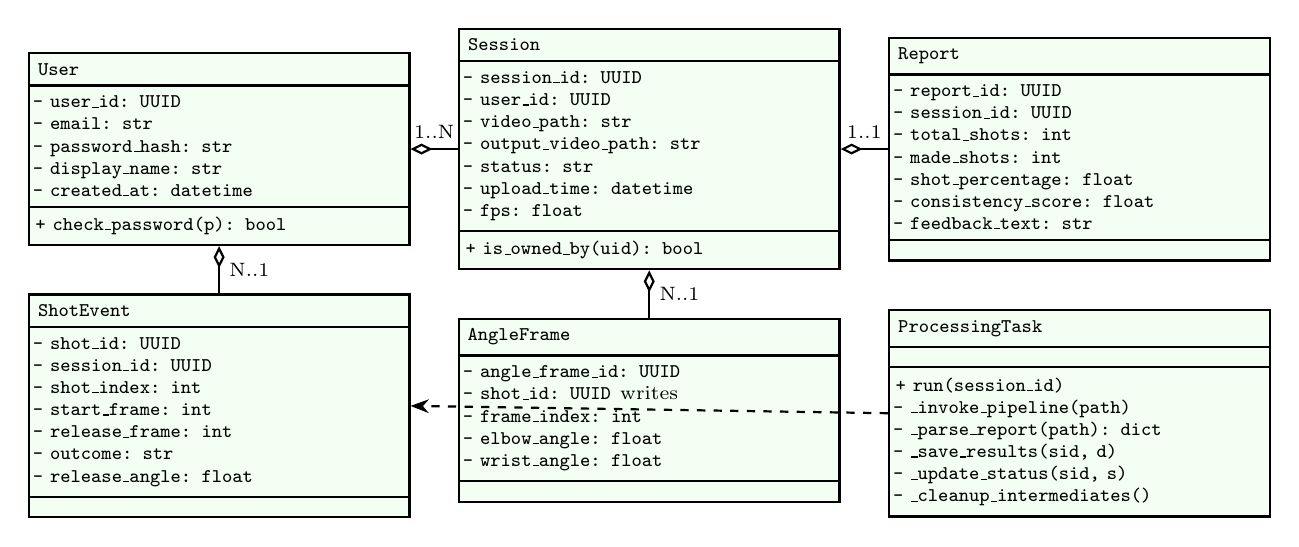
\begin{tikzpicture}[node distance=0.6cm and 0.6cm]
    \node[class] (user) {%
        \textbf{User} \nodepart{second}%
        - user\_id: UUID \\
        - email: str \\
        - password\_hash: str \\
        - display\_name: str \\
        - created\_at: datetime \nodepart{third}%
        + check\_password(p): bool
    };
    \node[class, right=of user] (sess) {%
        \textbf{Session} \nodepart{second}%
        - session\_id: UUID \\
        - user\_id: UUID \\
        - video\_path: str \\
        - output\_video\_path: str \\
        - status: str \\
        - upload\_time: datetime \\
        - fps: float \nodepart{third}%
        + is\_owned\_by(uid): bool
    };
    \node[class, right=of sess] (rep) {%
        \textbf{Report} \nodepart{second}%
        - report\_id: UUID \\
        - session\_id: UUID \\
        - total\_shots: int \\
        - made\_shots: int \\
        - shot\_percentage: float \\
        - consistency\_score: float \\
        - feedback\_text: str \nodepart{third}%
    };
    \node[class, below=of user] (shot) {%
        \textbf{ShotEvent} \nodepart{second}%
        - shot\_id: UUID \\
        - session\_id: UUID \\
        - shot\_index: int \\
        - start\_frame: int \\
        - release\_frame: int \\
        - outcome: str \\
        - release\_angle: float \nodepart{third}%
    };
    \node[class, below=of sess] (ang) {%
        \textbf{AngleFrame} \nodepart{second}%
        - angle\_frame\_id: UUID \\
        - shot\_id: UUID \\
        - frame\_index: int \\
        - elbow\_angle: float \\
        - wrist\_angle: float \nodepart{third}%
    };
    \node[class, below=of rep] (task) {%
        \textbf{ProcessingTask} \nodepart{second}%
        \nodepart{third}%
        + run(session\_id) \\
        - \_invoke\_pipeline(path) \\
        - \_parse\_report(path): dict \\
        - \_save\_results(sid, d) \\
        - \_update\_status(sid, s) \\
        - \_cleanup\_intermediates()
    };

    \draw[thick, -{Diamond[open]}] (sess.west) -- node[above, font=\scriptsize] {1..N} (user.east);
    \draw[thick, -{Diamond[open]}] (rep.west) -- node[above, font=\scriptsize] {1..1} (sess.east);
    \draw[thick, -{Diamond[open]}] (shot.north) -- node[right, font=\scriptsize] {N..1} (user.south -| shot.north);
    \draw[thick, -{Diamond[open]}] (ang.north) -- node[right, font=\scriptsize] {N..1} (sess.south -| ang.north);
    \draw[thick, dashed, -{Stealth}] (task.west) -- node[above, font=\scriptsize] {writes} (shot.east);
\end{tikzpicture}

\textit{Figure 3: Class Diagram (Web Layer)}
\end{center}

\paragraph{Existing pipeline classes} (reused unchanged): \texttt{BallTracker}, \texttt{RimTracker}, \texttt{HumanTracker}, \texttt{ShotTracker}, \texttt{BallTracksDrawer}, \texttt{RimTracksDrawer}, \texttt{HumanTracksDrawer}, and the utilities \texttt{read\_video}, \texttt{write\_video}, \texttt{ball\_hand}, \texttt{shot\_started}.

\subsubsection{Sequence Diagrams}

\textbf{Sequence 1: Video Upload and Processing}

\begin{center}
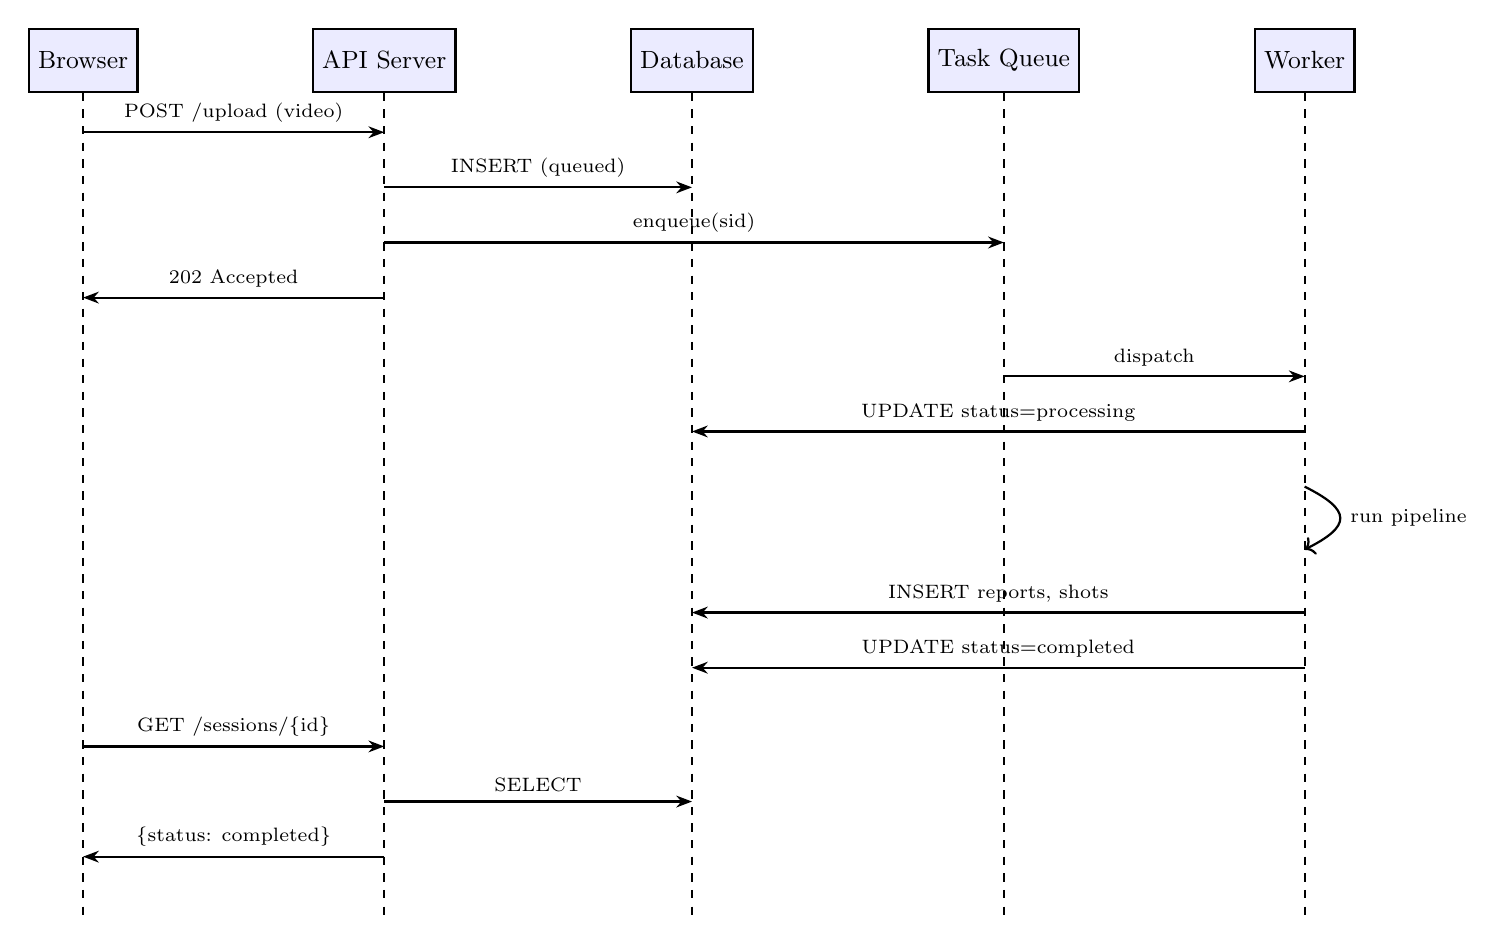
\begin{tikzpicture}[node distance=2.2cm]
    \node[box] (b) {Browser};
    \node[box, right=of b] (api) {API Server};
    \node[box, right=of api] (db) {Database};
    \node[box, right=of db] (q) {Task Queue};
    \node[box, right=of q] (w) {Worker};

    \foreach \n/\y in {b/-10.5, api/-10.5, db/-10.5, q/-10.5, w/-10.5} {
        \draw[lifeline] (\n.south) -- ($(\n.south)+(0,\y)$);
    }

    \draw[msg] ($(b.south)+(0,-0.5)$) -- node[above, font=\scriptsize] {POST /upload (video)} ($(api.south)+(0,-0.5)$);
    \draw[msg] ($(api.south)+(0,-1.2)$) -- node[above, font=\scriptsize] {INSERT (queued)} ($(db.south)+(0,-1.2)$);
    \draw[msg] ($(api.south)+(0,-1.9)$) -- node[above, font=\scriptsize] {enqueue(sid)} ($(q.south)+(0,-1.9)$);
    \draw[msg] ($(api.south)+(0,-2.6)$) -- node[above, font=\scriptsize] {202 Accepted} ($(b.south)+(0,-2.6)$);
    \draw[msg] ($(q.south)+(0,-3.6)$) -- node[above, font=\scriptsize] {dispatch} ($(w.south)+(0,-3.6)$);
    \draw[msg] ($(w.south)+(0,-4.3)$) -- node[above, font=\scriptsize] {UPDATE status=processing} ($(db.south)+(0,-4.3)$);
    \draw[->, thick] ($(w.south)+(0,-5.0)$) .. controls +(0.6,-0.3) and +(0.6,0.3) .. node[right, font=\scriptsize] {run pipeline} ($(w.south)+(0,-5.8)$);
    \draw[msg] ($(w.south)+(0,-6.6)$) -- node[above, font=\scriptsize] {INSERT reports, shots} ($(db.south)+(0,-6.6)$);
    \draw[msg] ($(w.south)+(0,-7.3)$) -- node[above, font=\scriptsize] {UPDATE status=completed} ($(db.south)+(0,-7.3)$);
    \draw[msg] ($(b.south)+(0,-8.3)$) -- node[above, font=\scriptsize] {GET /sessions/\{id\}} ($(api.south)+(0,-8.3)$);
    \draw[msg] ($(api.south)+(0,-9.0)$) -- node[above, font=\scriptsize] {SELECT} ($(db.south)+(0,-9.0)$);
    \draw[msg] ($(api.south)+(0,-9.7)$) -- node[above, font=\scriptsize] {\{status: completed\}} ($(b.south)+(0,-9.7)$);
\end{tikzpicture}

\textit{Figure 4: Sequence Diagram: Upload and Processing}
\end{center}

\textbf{Sequence 2: View Shot Analytics}

\begin{center}
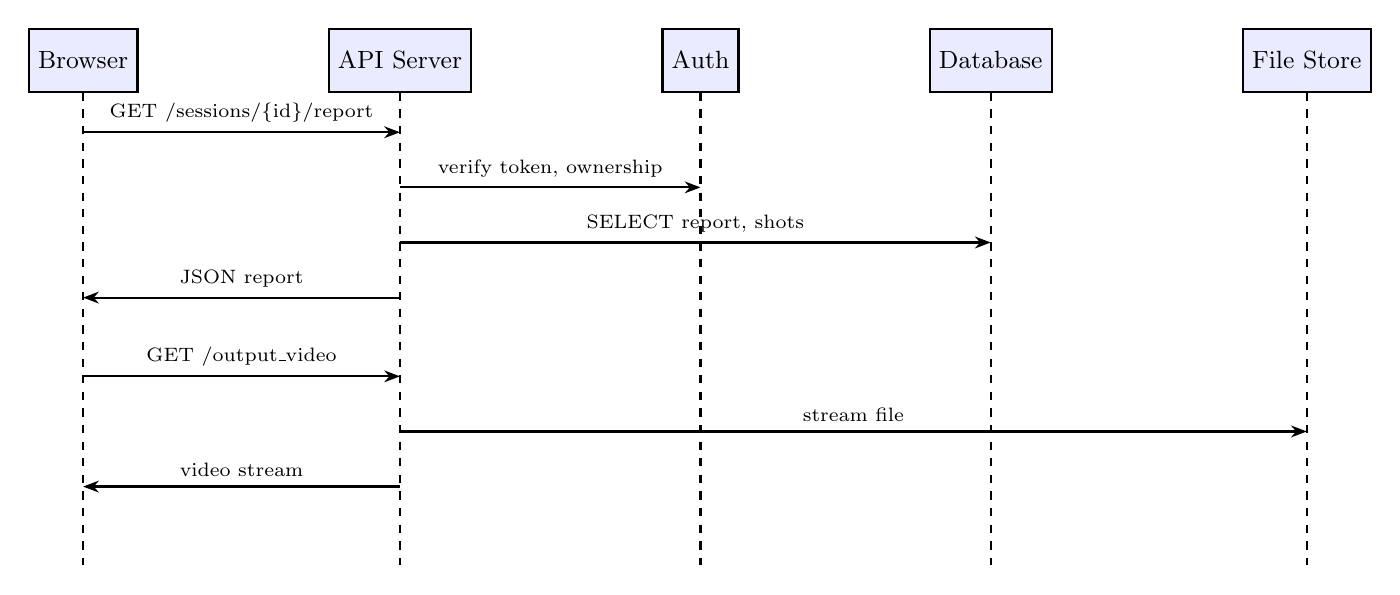
\begin{tikzpicture}[node distance=2.4cm]
    \node[box] (b) {Browser};
    \node[box, right=of b] (api) {API Server};
    \node[box, right=of api] (auth) {Auth};
    \node[box, right=of auth] (db) {Database};
    \node[box, right=of db] (fs) {File Store};

    \foreach \n in {b,api,auth,db,fs} \draw[lifeline] (\n.south) -- ($(\n.south)+(0,-6)$);

    \draw[msg] ($(b.south)+(0,-0.5)$) -- node[above, font=\scriptsize] {GET /sessions/\{id\}/report} ($(api.south)+(0,-0.5)$);
    \draw[msg] ($(api.south)+(0,-1.2)$) -- node[above, font=\scriptsize] {verify token, ownership} ($(auth.south)+(0,-1.2)$);
    \draw[msg] ($(api.south)+(0,-1.9)$) -- node[above, font=\scriptsize] {SELECT report, shots} ($(db.south)+(0,-1.9)$);
    \draw[msg] ($(api.south)+(0,-2.6)$) -- node[above, font=\scriptsize] {JSON report} ($(b.south)+(0,-2.6)$);
    \draw[msg] ($(b.south)+(0,-3.6)$) -- node[above, font=\scriptsize] {GET /output\_video} ($(api.south)+(0,-3.6)$);
    \draw[msg] ($(api.south)+(0,-4.3)$) -- node[above, font=\scriptsize] {stream file} ($(fs.south)+(0,-4.3)$);
    \draw[msg] ($(api.south)+(0,-5.0)$) -- node[above, font=\scriptsize] {video stream} ($(b.south)+(0,-5.0)$);
\end{tikzpicture}

\textit{Figure 5: Sequence Diagram: View Shot Analytics}
\end{center}

\subsubsection{State Diagrams}

\textbf{Session State Machine}

\begin{center}
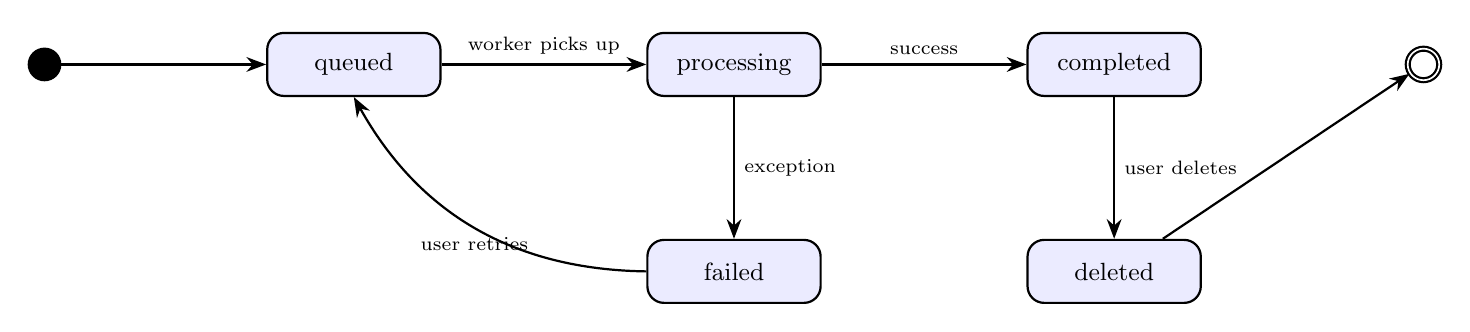
\begin{tikzpicture}[node distance=1.8cm and 2.6cm]
    \node[start] (s) {};
    \node[state, right=of s] (q) {queued};
    \node[state, right=of q] (p) {processing};
    \node[state, right=of p] (c) {completed};
    \node[state, below=of p] (f) {failed};
    \node[endst, right=of c] (e) {};
    \node[state, below=of c] (d) {deleted};

    \draw[flow] (s) -- (q);
    \draw[flow] (q) -- node[above, font=\scriptsize] {worker picks up} (p);
    \draw[flow] (p) -- node[above, font=\scriptsize] {success} (c);
    \draw[flow] (p) -- node[right, font=\scriptsize] {exception} (f);
    \draw[flow] (f.west) to[bend left=30] node[below, font=\scriptsize] {user retries} (q.south);
    \draw[flow] (c) -- node[right, font=\scriptsize] {user deletes} (d);
    \draw[flow] (d) -- (e);
\end{tikzpicture}

\textit{Figure 6: Session State Diagram}
\end{center}

\textbf{User Authentication State}

\begin{center}
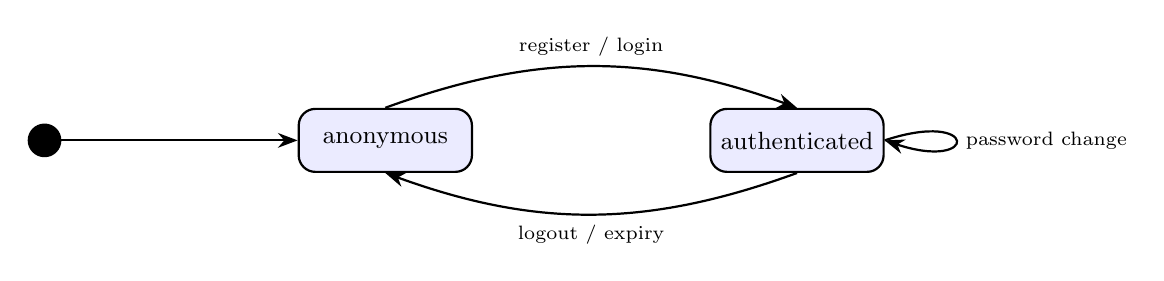
\begin{tikzpicture}[node distance=1.4cm and 3cm]
    \node[start] (s) {};
    \node[state, right=of s] (a) {anonymous};
    \node[state, right=of a] (au) {authenticated};

    \draw[flow] (s) -- (a);
    \draw[flow] (a.north) to[bend left=20] node[above, font=\scriptsize] {register / login} (au.north);
    \draw[flow] (au.south) to[bend left=20] node[below, font=\scriptsize] {logout / expiry} (a.south);
    \draw[flow] (au.east) .. controls +(1.2,0.4) and +(1.2,-0.4) .. node[right, font=\scriptsize] {password change} (au.east);
\end{tikzpicture}

\textit{Figure 7: Authentication State Diagram}
\end{center}

\subsubsection{Activity Diagrams}

\textbf{Full Pipeline Execution (Worker)}

\begin{center}
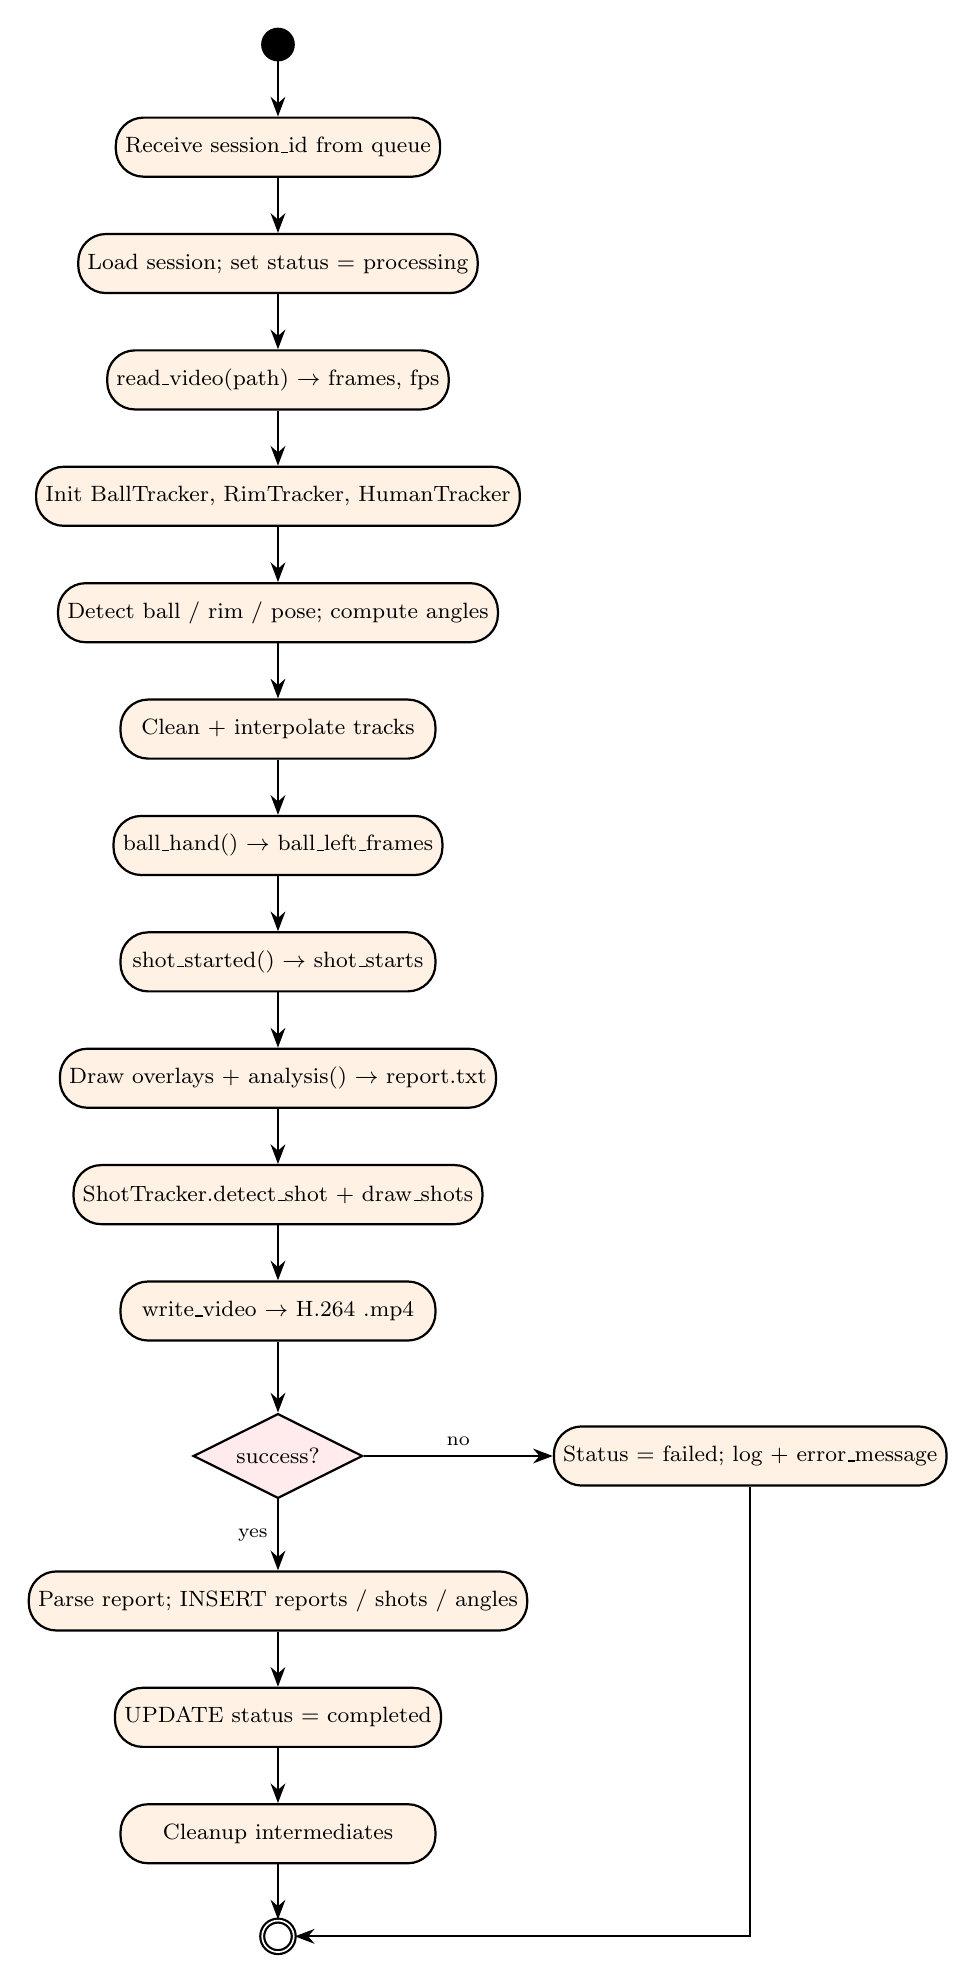
\begin{tikzpicture}[node distance=0.7cm]
    \node[start] (s) {};
    \node[activity, below=of s] (a1) {Receive session\_id from queue};
    \node[activity, below=of a1] (a2) {Load session; set status = processing};
    \node[activity, below=of a2] (a3) {read\_video(path) $\to$ frames, fps};
    \node[activity, below=of a3] (a4) {Init BallTracker, RimTracker, HumanTracker};
    \node[activity, below=of a4] (a5) {Detect ball / rim / pose; compute angles};
    \node[activity, below=of a5] (a6) {Clean + interpolate tracks};
    \node[activity, below=of a6] (a7) {ball\_hand() $\to$ ball\_left\_frames};
    \node[activity, below=of a7] (a8) {shot\_started() $\to$ shot\_starts};
    \node[activity, below=of a8] (a9) {Draw overlays + analysis() $\to$ report.txt};
    \node[activity, below=of a9] (a10) {ShotTracker.detect\_shot + draw\_shots};
    \node[activity, below=of a10] (a11) {write\_video $\to$ H.264 .mp4};
    \node[decision, below=of a11, yshift=-0.2cm] (d) {success?};
    \node[activity, below=of d, yshift=-0.2cm] (a12) {Parse report; INSERT reports / shots / angles};
    \node[activity, below=of a12] (a13) {UPDATE status = completed};
    \node[activity, below=of a13] (a14) {Cleanup intermediates};
    \node[activity, right=2.4cm of d] (af) {Status = failed; log + error\_message};
    \node[endst, below=of a14] (e) {};

    \foreach \x/\y in {s/a1, a1/a2, a2/a3, a3/a4, a4/a5, a5/a6, a6/a7, a7/a8, a8/a9, a9/a10, a10/a11, a11/d} \draw[flow] (\x) -- (\y);
    \draw[flow] (d) -- node[left, font=\scriptsize] {yes} (a12);
    \draw[flow] (a12) -- (a13);
    \draw[flow] (a13) -- (a14);
    \draw[flow] (a14) -- (e);
    \draw[flow] (d) -- node[above, font=\scriptsize] {no} (af);
    \draw[flow] (af.south) |- (e.east);
\end{tikzpicture}

\textit{Figure 8: Pipeline Activity Diagram}
\end{center}

\textbf{User Registration}

\begin{center}
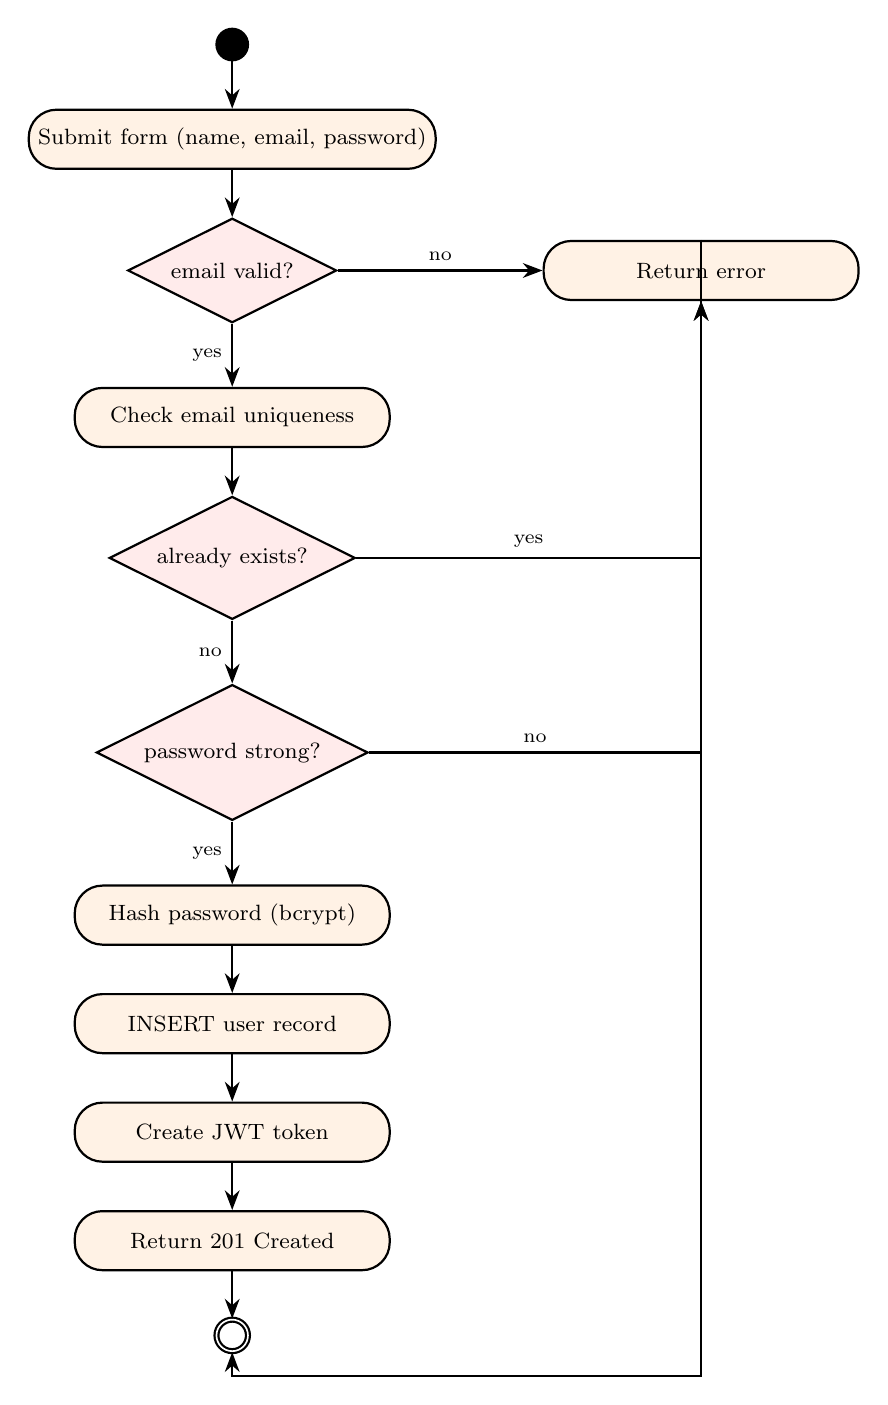
\begin{tikzpicture}[node distance=0.6cm]
    \node[start] (s) {};
    \node[activity, below=of s] (a1) {Submit form (name, email, password)};
    \node[decision, below=of a1] (d1) {email valid?};
    \node[activity, below=of d1, yshift=-0.2cm] (a2) {Check email uniqueness};
    \node[decision, below=of a2] (d2) {already exists?};
    \node[decision, below=of d2, yshift=-0.2cm] (d3) {password strong?};
    \node[activity, below=of d3, yshift=-0.2cm] (a3) {Hash password (bcrypt)};
    \node[activity, below=of a3] (a4) {INSERT user record};
    \node[activity, below=of a4] (a5) {Create JWT token};
    \node[activity, below=of a5] (a6) {Return 201 Created};
    \node[endst, below=of a6] (e) {};
    \node[activity, right=2.6cm of d1] (err1) {Return error};

    \draw[flow] (s) -- (a1);
    \draw[flow] (a1) -- (d1);
    \draw[flow] (d1) -- node[left, font=\scriptsize] {yes} (a2);
    \draw[flow] (a2) -- (d2);
    \draw[flow] (d2) -- node[left, font=\scriptsize] {no} (d3);
    \draw[flow] (d3) -- node[left, font=\scriptsize] {yes} (a3);
    \draw[flow] (a3) -- (a4);
    \draw[flow] (a4) -- (a5);
    \draw[flow] (a5) -- (a6);
    \draw[flow] (a6) -- (e);
    \draw[flow] (d1) -- node[above, font=\scriptsize] {no} (err1);
    \draw[flow] (d2.east) -| node[above, font=\scriptsize, pos=0.25] {yes} (err1.south);
    \draw[flow] (d3.east) -| node[above, font=\scriptsize, pos=0.25] {no} (err1.south);
    \draw[flow] (err1.north) |- ($(e.south)+(0,-0.3)$) -| (e.south);
\end{tikzpicture}

\textit{Figure 9: Registration Activity Diagram}
\end{center}

\subsubsection{System User Interface}

\textbf{Screen 1: Dashboard / Home}

\begin{center}
\includegraphics[width=\linewidth,keepaspectratio]{dashboard.png}

\textit{Figure 10: Dashboard}
\end{center}

\textbf{Screen 2: Upload Page}

\begin{center}
\includegraphics[width=\linewidth,keepaspectratio]{upload.png}

\textit{Figure 11: Upload}
\end{center}

\textbf{Screen 3: Session Results: Shot Analytics}

\begin{center}
\includegraphics[width=\linewidth,keepaspectratio]{shot_analytics.png}

\textit{Figure 12: Shot Analytics}
\end{center}

\textbf{Screen 4: Session Results: Form Analysis}

\begin{center}
\includegraphics[width=0.7\linewidth,keepaspectratio]{form_analysis.png}

\textit{Figure 13: Form Analysis}
\end{center}

\textbf{Screen 5: Session History}

\begin{center}
\includegraphics[width=\linewidth,keepaspectratio]{sessionHistory.png}

\textit{Figure 14: Session History}
\end{center}

\section{References}
\begin{itemize}[leftmargin=*]
    \item Project SRS: SwishVision Software Requirements Specification v1.10
    \item Ultralytics YOLOv8 Documentation: \url{https://docs.ultralytics.com}
    \item Existing codebase: \texttt{main.py}, \texttt{trackers/}, \texttt{drawers/}, \texttt{utils/}
\end{itemize}

\section{Appendices}

\subsection*{Appendix A: API Endpoint Summary}

\begin{longtable}{|c|L{6cm}|c|L{5cm}|}
\hline
\textbf{Method} & \textbf{Endpoint} & \textbf{Auth} & \textbf{Description} \\ \hline
POST & \texttt{/api/register} & No & Create new user account \\ \hline
POST & \texttt{/api/login} & No & Authenticate and receive token \\ \hline
POST & \texttt{/api/logout} & Yes & Invalidate current session \\ \hline
POST & \texttt{/api/sessions/upload} & Yes & Upload a video for processing \\ \hline
GET & \texttt{/api/sessions} & Yes & List sessions for user \\ \hline
GET & \texttt{/api/sessions/\{id\}} & Yes & Get session status / metadata \\ \hline
DELETE & \texttt{/api/sessions/\{id\}} & Yes & Delete a session and its data \\ \hline
GET & \texttt{/api/sessions/\{id\}/report} & Yes & Get full report data \\ \hline
GET & \texttt{/api/sessions/\{id\}/shots} & Yes & Get all shot events \\ \hline
GET & \texttt{/api/sessions/\{id\}/output\_video} & Yes & Stream annotated video \\ \hline
GET & \texttt{/api/dashboard/summary} & Yes & Aggregate stats for user \\ \hline
GET & \texttt{/api/dashboard/trends} & Yes & Historical trend data \\ \hline
\end{longtable}

\subsection*{Appendix B: File System Layout}

\begin{lstlisting}
Swish-Vision/                        # Project root
|-- main.py                          # Pipeline entry point
|-- trackers/                        # BallTracker, RimTracker, HumanTracker
|-- drawers/                         # Drawer modules + ShotTracker
|-- utils/                           # vid_utils.py, ball_hand.py, stubs_utils.py
|-- models/                          # best.pt, yolov8m-pose.pt
|-- input_videos/                    # Worker copies uploaded video here
|-- output_videos/                   # Pipeline writes H.264 .mp4 output here
|-- reports/                         # Pipeline writes {vidname}_report.txt
|-- Basketball-1/                    # Training dataset
|-- runs/                            # YOLO training run history
|-- app/                             # Web application layer (delivered)
    |-- main.py                      # FastAPI app factory + lifespan
    |-- config.py                    # Pydantic Settings (.env)
    |-- database.py                  # SQLAlchemy engine + SessionLocal
    |-- api/
    |   |-- auth.py
    |   |-- sessions.py
    |   |-- dashboard.py
    |-- core/
    |   |-- security.py              # bcrypt + JWT helpers
    |   |-- middleware.py            # CORS, security headers
    |-- models/                      # SQLAlchemy ORM models
    |-- schemas/                     # Pydantic request/response schemas
    |-- tasks/
    |   |-- pipeline_task.py         # Celery app + process_video task
    |   |-- report_parser.py
    |-- migrations/                  # Alembic
    |-- frontend/                    # React (Create React App)
    |-- uploads/                     # Raw user-uploaded videos
    |-- requirements.txt
    |-- DEVELOPER_README.md
\end{lstlisting}

\subsection*{Appendix C: Environment Variables}

\begin{longtable}{|L{5cm}|L{9cm}|}
\hline
\textbf{Variable} & \textbf{Description} \\ \hline
\texttt{ENV} & Environment name: \texttt{development} / \texttt{staging} / \texttt{production} \\ \hline
\texttt{DB\_SERVER} & SQL Server hostname/instance \\ \hline
\texttt{DB\_NAME} & SQL Server database name \\ \hline
\texttt{DB\_DRIVER} & ODBC driver name (e.g. ODBC Driver 17 for SQL Server) \\ \hline
\texttt{DB\_TRUSTED\_CONNECTION} & \texttt{true} for Windows auth; else use DB\_USERNAME/PASSWORD \\ \hline
\texttt{DB\_USERNAME} / \texttt{DB\_PASSWORD} & SQL auth credentials \\ \hline
\texttt{REDIS\_URL} & Redis connection string for Celery broker \\ \hline
\texttt{CELERY\_RESULT\_BACKEND} & Celery result backend URL \\ \hline
\texttt{SECRET\_KEY} & JWT signing secret \\ \hline
\texttt{ADMIN\_RESET\_KEY} & Shared secret for admin force-reset endpoint \\ \hline
\texttt{UPLOAD\_DIR} & Path for raw uploaded videos \\ \hline
\texttt{OUTPUT\_DIR} & Path for annotated H.264 \texttt{.mp4} outputs \\ \hline
\texttt{MODEL\_DIR} & Path to YOLOv8 model weights \\ \hline
\texttt{MAX\_UPLOAD\_SIZE\_MB} & Maximum allowed upload size (default 500) \\ \hline
\end{longtable}

\end{document}
